\documentclass[11pt, a4paper]{article}
\usepackage{sectsty}
\usepackage{enumitem}
\usepackage{graphicx}
\usepackage{amsmath}
\usepackage{amssymb}
\usepackage{setspace}
\usepackage{tasks}
\usepackage{graphicx}
\usepackage{float}
\usepackage{comment}
\usepackage{listings}
\usepackage[utf8]{inputenc}
\usepackage{amsfonts}
\usepackage{gensymb}
\usepackage{multicol}
\usepackage{tabularx}
\usepackage{tikz}
\newcommand{\myvec}[1]{\ensuremath{\begin{pmatrix}#1\end{pmatrix}}}
\let\vec\mathbf

\newcommand{\mydet}[1]{\ensuremath{\begin{vmatrix}#1\end{vmatrix}}}
\providecommand{\brak}[1]{\ensuremath{\left(#1\right)}}
\providecommand{\lbrak}[1]{\ensuremath{\left(#1\right.}}
\providecommand{\rbrak}[1]{\ensuremath{\left.#1\right)}}
\providecommand{\cbrak}[1]{\ensuremath{\left\{#1\right\}}}
\providecommand{\sbrak}[1]{\ensuremath{{}\left[#1\right]}}
\providecommand{\norm}[1]{\left\lVert#1\right\rVert}
\providecommand{\abs}[1]{\left\vert#1\right\vert}

\title{ \textbf{Math Computing}}
\date{}

\begin{document}
\vspace{-\baselineskip}
\maketitle

\section*{NCERT 9.7.1.6}

\textbf{This question is from class 9 NCERT chapter 7.triangles}
\begin{enumerate}
\item $\vec{AC} = \vec{AE}$ , $\vec{AB} = \vec{AD}$ and $\angle BAD = \angle EAC$. Show that$\vec{BC} = \vec{DE}$
	
\begin{figure}[H]
    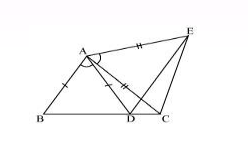
\includegraphics[width=\columnwidth]{figs/ABCDE.png}
	\caption{$\triangle  \vec{ABC} \hspace{12pt} and \hspace{12pt} \triangle \vec{ADE}$}
 \label{fig:fig1}
\end{figure}
\pagebreak
\textbf{Construction steps:}
\\
		\begin{enumerate}[label=(\roman*)]

\item Let assume, the input parameters are, 
\begin{table}[H]
\centering
	\begin{tabular}{|c|c|p{5cm}|}
\hline
\textbf{Parameter} & \textbf{Value} & \textbf{Description} \\
\hline
	$\theta$ & $60\degree$ & $\angle{BAD} = \angle{CAE}$ \\
\hline
	$\vec{B}$ & $\myvec{0\\0}$ & Reference point at origin \\
\hline
	$\vec{D}$ & $\myvec{6\\0}$ & point $\vec{D}$ on the same axis of $\vec{B}$ \\
\hline
	$\vec{C}$ & $\myvec{8\\0}$ & point $\vec{C}$ on the same axis of $\vec{B}$ \\
\hline

\end{tabular}

	  \caption{Input Parameters}
	  \label{Table-1: }
\end{table}

$\therefore$ the output can be calculated as,
\begin{table}[H]
\centering
	\begin{tabular}{|c|c|p{5cm}|}
\hline
\textbf{Parameter} & \textbf{Value} & \textbf{Description} \\
\hline
	$r1$ & $\norm{B-D}$ & Length of $\vec{BD}$ \\
\hline
	$\vec{A}$ & $\vec{D}$ + $\myvec{-r1 \cos \theta  \\ r1 \sin \theta}$ & From point $\vec{D}$ makes an angle $\theta$ in clock-wise with line $\vec{(AD, AB)}$  \\
\hline
	  
	$r1$ & $\norm{B-D}$ & Length of $\vec{BD}$ \\
\hline       
	$\vec{E}$ & $\vec{D}$ + $\myvec{r2 \cos \theta  \\ r2 \sin \theta}$ & From point $\vec{D}$ makes an angle $\theta$ in anticlock-wise with line $\vec{(AC, CE)}$  \\  
\hline

\end{tabular}

	  \caption{Output Parameters}
	  \label{Table-2: }
\end{table}

$\therefore$ By, joining these points forms the required figure

\end{enumerate}
\begin{figure}[H]
    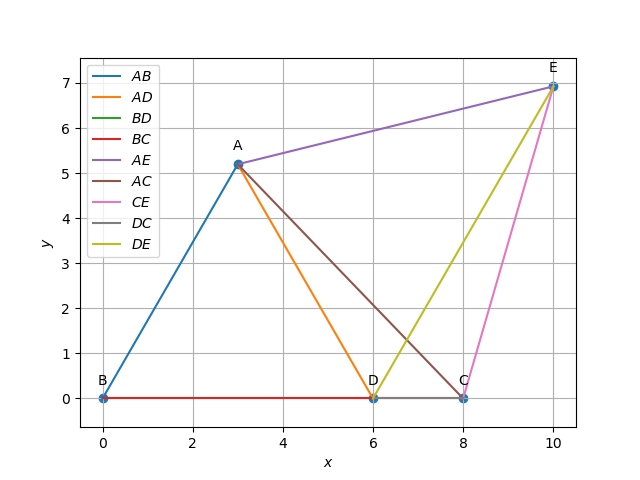
\includegraphics[width=\columnwidth]{figs/Final_python.png}
	\caption{$\triangle \vec{ABC} \hspace{12pt} and \hspace{12pt} \triangle \vec{ADE}$}
    \label{fig:fig2}
\end{figure}
\end{enumerate}

\end{document} 
